Initially, we make the load station size 4. Then by statistics, we've found that there are about \%2.7 of the time the load station is full. There might be potential for more load to be waiting in the load station at the same time, which can make memory request happens earlier and then improve the CPI. Therefore, we initiate a load station size optimization. We've attempted to change the size of the load station to fully leverage its potential in improving the performance. Here we changed the size from 1 to 5. And we are recording the normalized performance, which is calculated by \ref{eq:load_size}. We are all comparing with the situation of size 4. 

\begin{equation}
\text{Normalized Performance}_i=\frac{\text{CPI}_{\text{N=4}}}{\text{CPI}_{\text{N=i}}} 
\label{eq:load_size}
\end{equation}


From Fig. \ref{fig:load_size} we can see that the performance improved dramatically whenthe  size changes from 1 to 3. However, there's almost no improvement when the size changes from 4 to 5. Since load station is not on the critical path, there's no need to make it smaller. Finally, we just keep it at the size of 4. We have already exploited its potential. 


\begin{figure}[htbp]
\centerline{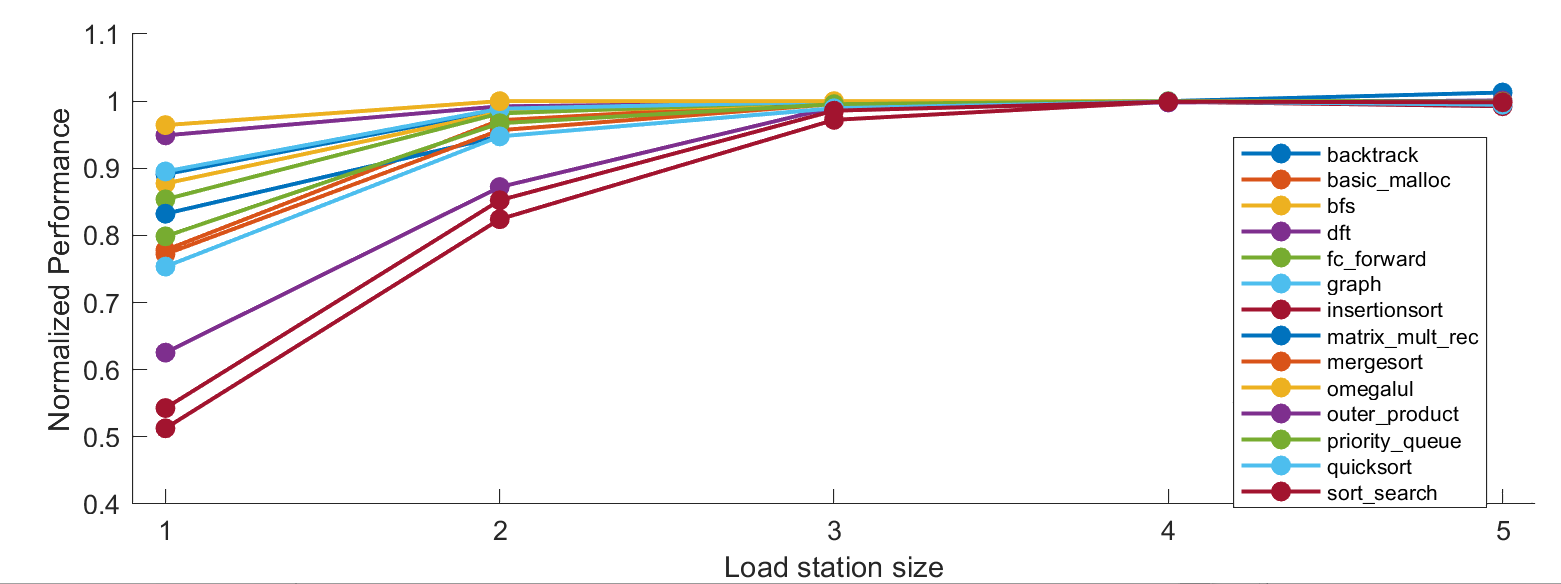
\includegraphics[width=0.5\textwidth]{figures/Analysis/load_size.png}}
\caption{Performance vs load station size.}
\label{fig:load_size}
\end{figure}